\documentclass[12pt,a4paper]{article}

% ─── Page Layout ───────────────────────────────────────────────────────────────
\usepackage[a4paper, margin=0.8in, headheight=14pt]{geometry}

% ─── Fonts (XeLaTeX) ───────────────────────────────────────────────────────────
\usepackage{fontspec}
\usepackage{unicode-math}
\setmainfont{TeX Gyre Pagella}
\setmonofont[Scale=0.88]{TeX Gyre Cursor}
\setmathfont{Latin Modern Math}

% ─── Packages ──────────────────────────────────────────────────────────────────
\usepackage{xcolor}
\usepackage{colortbl}
\usepackage{titlesec}
\usepackage{enumitem}
\usepackage{tabularx}
\usepackage{booktabs}
\usepackage{array}
\usepackage{amsmath}
\usepackage{tikz}
\usetikzlibrary{shapes.geometric, arrows.meta, positioning, calc, fit, decorations.pathreplacing}
\usepackage{tcolorbox}
\tcbuselibrary{skins, breakable}
\usepackage{hyperref}
\usepackage{fancyhdr}
\usepackage{graphicx}
\usepackage{microtype}
\hyphenpenalty=10000
\exhyphenpenalty=10000
\sloppy
\usepackage{caption}
\usepackage{setspace}
\usepackage{multirow}
\usepackage{tocloft}

% ─── Q&A helper ────────────────────────────────────────────────────────────────
\newcommand{\Q}[1]{\textbf{#1}\par\noindent\ignorespaces}

% ─── Colour Palette ────────────────────────────────────────────────────────────
\definecolor{myred}{RGB}{196,30,58}
\definecolor{mydark}{RGB}{30,30,50}
\definecolor{mygreen}{RGB}{14,120,80}
\definecolor{myteal}{RGB}{0,130,140}
\definecolor{myamber}{RGB}{180,100,0}
\definecolor{mypurple}{RGB}{100,30,160}
\definecolor{mygray}{RGB}{246,247,249}
\definecolor{mgframe}{RGB}{180,185,200}
\definecolor{watermark}{RGB}{145,150,170}
\definecolor{hdrred}{RGB}{250,232,235}
\definecolor{hdrgreen}{RGB}{220,244,233}
\definecolor{hdrteal}{RGB}{220,242,244}
\definecolor{hdramber}{RGB}{253,242,215}
\definecolor{hdrpurple}{RGB}{238,228,255}
\definecolor{hdrgray}{RGB}{238,240,245}
\definecolor{rowalt}{RGB}{250,251,253}

% ─── Section Formatting ────────────────────────────────────────────────────────
\titleformat{\section}
  {\large\bfseries\color{myred}}{\thesection.}{0.5em}{}
  [\vspace{1pt}{\color{myred}\rule{\linewidth}{0.8pt}}]
\titleformat{\subsection}
  {\normalsize\bfseries\color{myteal}}{\thesubsection}{0.5em}{}
\titlespacing*{\section}{0pt}{18pt}{7pt}
\titlespacing*{\subsection}{0pt}{11pt}{4pt}

% ─── Paragraph ─────────────────────────────────────────────────────────────────
\setlength{\parindent}{0pt}
\setlength{\parskip}{4pt}

% ─── TOC Styling ───────────────────────────────────────────────────────────────
\renewcommand{\cfttoctitlefont}{\large\bfseries\color{myred}}
\renewcommand{\cftaftertoctitle}{\par\noindent{\color{myred}\rule{\linewidth}{0.8pt}}}
\setlength{\cftbeforetoctitleskip}{0pt}
\setlength{\cftaftertoctitleskip}{6pt}
\renewcommand{\cftsecfont}{\normalsize\bfseries\color{mydark}}
\renewcommand{\cftsecpagefont}{\normalsize\bfseries\color{mydark}}
\renewcommand{\cftsecleader}{\cftdotfill{\cftdotsep}}
\setlength{\cftbeforesecskip}{7pt}
\renewcommand{\cftsubsecfont}{\small\color{mydark}}
\renewcommand{\cftsubsecpagefont}{\small\color{mydark}}
\setlength{\cftbeforesubsecskip}{3pt}
\setlength{\cftsubsecindent}{1.4em}

% ─── Table helpers ─────────────────────────────────────────────────────────────
\renewcommand{\arraystretch}{1.45}
\setlength{\tabcolsep}{6pt}
\arrayrulecolor{mydark}
\newcolumntype{B}[1]{>{\small\bfseries\raggedright\arraybackslash}m{#1}}
\newcolumntype{Y}{>{\small\raggedright\arraybackslash}X}
\renewcommand{\tabularxcolumn}[1]{m{#1}}

% ─── Header / Footer ───────────────────────────────────────────────────────────
\pagestyle{fancy}
\fancyhf{}
\fancyhead[L]{\small\color{myred}\textbf{OE-EC704C}\;\color{mydark}--- Entrepreneurship}
\fancyhead[R]{\small\color{myteal}\textbf{Module 4 Notes}}
\fancyfoot[C]{\small\color{mydark}\thepage}
\fancyfoot[R]{\small\color{watermark}\textit{\copyright\ Biraj}}
\renewcommand{\headrulewidth}{0.5pt}
\renewcommand{\footrulewidth}{0.3pt}

% ─── Hyperref ──────────────────────────────────────────────────────────────────
\hypersetup{
  colorlinks=true, linkcolor=myteal, urlcolor=myteal,
  pdfauthor={Biraj Sarkar},
  pdftitle={OE-EC704C --- Module 4 Notes}
}

% ─── tcolorbox styles ──────────────────────────────────────────────────────────
\tcbset{
  tikzbox/.style={
    colback=mygray, colframe=mgframe, boxrule=0.6pt, arc=4pt,
    left=8pt, right=8pt, top=6pt, bottom=6pt,
    colbacktitle=mgframe, coltitle=mydark,
    fonttitle=\small\bfseries
  },
  defbox/.style={
    colback=hdrgreen, colframe=mygreen, boxrule=0.8pt, arc=4pt,
    left=9pt, right=9pt, top=6pt, bottom=6pt,
    colbacktitle=mygreen, coltitle=white,
    fonttitle=\small\bfseries
  },
  formulabox/.style={
    colback=hdrteal, colframe=myteal, boxrule=0.8pt, arc=4pt,
    left=9pt, right=9pt, top=7pt, bottom=7pt,
    colbacktitle=myteal, coltitle=white,
    fonttitle=\small\bfseries
  },
  examplebox/.style={
    colback=hdramber, colframe=myamber, boxrule=0.8pt, arc=4pt,
    left=9pt, right=9pt, top=6pt, bottom=6pt,
    colbacktitle=myamber, coltitle=white,
    fonttitle=\small\bfseries
  },
  masonbox/.style={
    colback=hdrpurple, colframe=mypurple, boxrule=0.8pt, arc=4pt,
    left=9pt, right=9pt, top=6pt, bottom=6pt,
    colbacktitle=mypurple, coltitle=white,
    fonttitle=\small\bfseries
  },
  exambox/.style={
    colback=hdrpurple, colframe=mypurple, boxrule=1pt, arc=5pt,
    left=10pt, right=10pt, top=8pt, bottom=8pt,
    colbacktitle=mypurple, coltitle=white,
    fonttitle=\bfseries,
    breakable, title after break={\textbf{Frequently Asked / Viva Questions (contd.)}}}
}
\tcbset{breakable}

% ─── TikZ styles ───────────────────────────────────────────────────────────────
\tikzset{
  block/.style={rectangle, draw=myteal, fill=hdrteal,
    text width=2.4cm, align=center, minimum height=0.95cm,
    font=\small, rounded corners=3pt, line width=0.7pt},
  redblock/.style={rectangle, draw=myred, fill=hdrred,
    text width=2.4cm, align=center, minimum height=0.95cm,
    font=\small, rounded corners=3pt, line width=0.7pt},
  netnode/.style={rectangle, draw=myteal, fill=hdrteal,
    text width=1.5cm, align=center, minimum height=0.8cm,
    font=\small, rounded corners=3pt, line width=0.7pt},
  sumjunc/.style={circle, draw=myamber, fill=hdramber,
    minimum size=0.62cm, font=\small, line width=0.8pt},
  snode/.style={circle, draw=mypurple, fill=hdrpurple,
    minimum size=0.55cm, font=\footnotesize, line width=0.7pt},
  arrow/.style={-Stealth, thick, color=mydark},
  redarrow/.style={-Stealth, thick, color=myred},
  line/.style={thick, color=mydark}
}

% ═══════════════════════════════════════════════════════════════════════════════
\begin{document}
% ═══════════════════════════════════════════════════════════════════════════════

\begin{center}
  {\LARGE\bfseries\color{myred} OE-EC704C --- Entrepreneurship}\\[5pt]
  {\normalsize\color{mydark} Semester VII \quad$\bullet$\quad 3L:0T:0P \quad$\bullet$\quad 3 Credits}\\[3pt]
  {\normalsize\color{myteal}\textbf{Module 4 Exam Notes: Decision Making, Motivation \& Project Reports}}\\[3pt]
  {\small\color{mydark} CGEC \;$|$\; B.Tech ECE (2023--27) \;$|$\; \textit{Biraj Sarkar}}
\end{center}
\vspace{2pt}
\noindent{\color{myred}\rule{\linewidth}{1.5pt}}
\vspace{2pt}

\hypersetup{linkcolor=mydark}
\tableofcontents
\hypersetup{linkcolor=myteal}
\newpage

% ===============================================================================
\section{Decision Making in Management}
% ===============================================================================

\subsection{Meaning and Types of Decisions}
\begin{tcolorbox}[defbox, title={Definition of Decision Making}]
\textbf{Decision Making} is the cognitive process of identifying and selecting a course of action from among several alternatives to solve a specific problem or achieve a desired organizational goal.
\end{tcolorbox}

Managers classify decisions into several core topologies:
\begin{itemize}[leftmargin=*, itemsep=3.5pt]
  \item \textbf{Programmed vs. Non-Programmed Decisions:}
    \begin{itemize}[label=\tiny$\bullet$, leftmargin=1.5em, itemsep=1.5pt]
      \item \textit{Programmed:} Routine, repetitive decisions handled through established rules, policies, or procedures (e.g., reordering inventory when it hits a reorder level).
      \item \textit{Non-Programmed:} Unique, unstructured, and complex decisions requiring custom problem-solving, strategic judgment, and creative thinking (e.g., launching a new product line).
    \end{itemize}
  \item \textbf{Strategic vs. Operational Decisions:}
    \begin{itemize}[label=\tiny$\bullet$, leftmargin=1.5em, itemsep=1.5pt]
      \item \textit{Strategic:} High-stake, long-term decisions made by top management affecting the entire organization (e.g., expanding into international markets).
      \item \textit{Operational:} Short-term, day-to-day decisions made by lower-level managers to ensure smooth daily processes (e.g., scheduling worker shifts).
    \end{itemize}
\end{itemize}

\subsection{The Rational Decision-Making Process}
Rational decision-making involves 7 sequential steps:
$$\text{Identify Problem} \rightarrow \text{Gather Info} \rightarrow \text{Develop Alternatives} \rightarrow \text{Evaluate Options} \rightarrow \text{Select Choice} \rightarrow \text{Implement} \rightarrow \text{Review \& Feedback}$$

% ===============================================================================
\section{Forecasting Methodologies}
% ===============================================================================

Forecasting is the process of predicting future events or demands based on historical data and analytical models. It is critical for planning production, inventory, and finances.

\subsection{Qualitative vs. Quantitative Forecasting}
\par\noindent
{\renewcommand{\arraystretch}{1.5}%
\begin{tabularx}{\linewidth}{|B{3.0cm}|Y|Y|}\hline
\multicolumn{1}{|>{\centering\arraybackslash}m{3.0cm}|}{\textbf{Feature}} &
\multicolumn{1}{>{\centering\arraybackslash}Y|}{\textbf{Qualitative Methods}} &
\multicolumn{1}{>{\centering\arraybackslash}Y|}{\textbf{Quantitative Methods}} \\
\hline
\textbf{Basis} & Subjective judgment, intuition, and expert opinions. & Mathematical models and historical numerical data. \\
\hline
\textbf{Context} & Used when historical data is unavailable (e.g., new products). & Used when stable historical data is available (e.g., mature products). \\
\hline
\textbf{Key Techniques} & Delphi method, Jury of Executive Opinion, Sales Force Composite. & Time-Series models (moving averages, exponential smoothing), Regression models. \\
\hline
\textbf{Cost \& Accuracy} & Highly subjective; variable long-term accuracy. & Highly objective; reliable short-term mathematical accuracy. \\
\hline
\end{tabularx}
}

\subsection{Key Forecasting Techniques}
\begin{itemize}[leftmargin=*, itemsep=3.5pt]
  \item \textbf{Delphi Method (Qualitative):} A structured communication technique where a panel of experts answers questionnaires in two or more rounds. After each round, a facilitator provides an anonymous summary of the experts' forecasts and reasons. Experts are encouraged to revise their earlier answers, converging toward a consensus.
  \item \textbf{Simple Moving Average (Quantitative):} Predicts demand for the next period ($F_{t+1}$) by averaging the actual demand ($A_t$) over a fixed number of past periods ($n$):
    \begin{equation}
      F_{t+1} = \frac{A_t + A_{t-1} + \dots + A_{t-n+1}}{n}
    \end{equation}
  \item \textbf{Exponential Smoothing (Quantitative):} A weighted moving average method where recent data is weighted more heavily. The forecast ($F_{t+1}$) is calculated using the smoothing constant $\alpha$ ($0 \le \alpha \le 1$):
    \begin{equation}
      F_{t+1} = F_t + \alpha (A_t - F_t) = \alpha A_t + (1 - \alpha) F_t
    \end{equation}
\end{itemize}

% ===============================================================================
\section{Personnel Management}
% ===============================================================================

\subsection{Meaning and Core Functions}
\begin{tcolorbox}[defbox, title={Definition of Personnel Management}]
\textbf{Personnel Management} (often structured as Human Resource Management) is the function within an organization concerned with the recruitment, selection, development, utilization, and welfare of employees to align individual efforts with corporate objectives.
\end{tcolorbox}

The manager executes five core personnel functions:
\begin{enumerate}[label=\textbf{\arabic*.}, leftmargin=*, itemsep=3.5pt]
  \item \textbf{Recruitment:} Attracting a pool of qualified job candidates from internal or external sources.
  \item \textbf{Selection:} Assessing and choosing the best candidates using tests, interviews, and reference checks.
  \item \textbf{Training and Development:} Enhancing employee skills and capabilities through orientation, on-the-job training, and workshops.
  \item \textbf{Performance Appraisal:} Systematic evaluation of employee performance against set standards to determine raises, promotions, or training needs.
  \item \textbf{Compensation \& Welfare:} Designing fair salary structures, benefits, health insurance, and workplace safety measures.
\end{enumerate}

% ===============================================================================
\section{Theories of Motivation}
% ===============================================================================

Motivation is the inner state that energizes, directs, and sustains human behavior toward achieving organizational goals.

\subsection{Maslow's Need Hierarchy Theory}
Abraham Maslow (1943) proposed that human needs are structured in a strict hierarchy of five levels. A person satisfies lower-level needs before higher-level needs become active drivers of behavior. Once a need is satisfied, it ceases to motivate.

\begin{tcolorbox}[tikzbox, title={Maslow's Pyramid of Human Needs}]
\centering
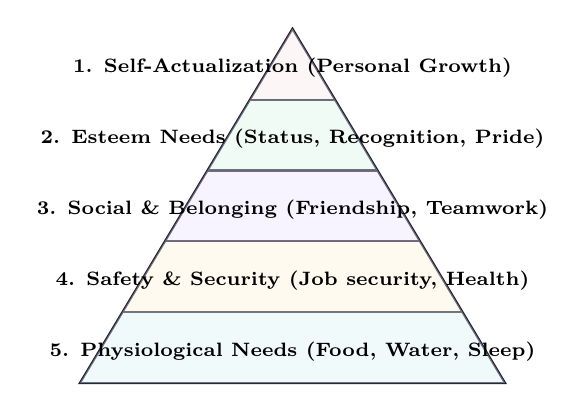
\begin{tikzpicture}[scale=0.9]
  % Triangle Coordinates
  \coordinate (A) at (0,0);
  \coordinate (B) at (6,0);
  \coordinate (C) at (3,5);
  
  \draw[thick, color=mydark] (A) -- (B) -- (C) -- cycle;
  
  % Level 5 (Physiological)
  \draw[thick, color=mydark] (0.6,1) -- (5.4,1);
  \fill[hdrteal, opacity=0.4] (0,0) -- (6,0) -- (5.4,1) -- (0.6,1) -- cycle;
  \node[font=\scriptsize\bfseries] at (3,0.45) {5. Physiological Needs (Food, Water, Sleep)};
  
  % Level 4 (Safety)
  \draw[thick, color=mydark] (1.2,2) -- (4.8,2);
  \fill[hdramber, opacity=0.4] (0.6,1) -- (5.4,1) -- (4.8,2) -- (1.2,2) -- cycle;
  \node[font=\scriptsize\bfseries] at (3,1.45) {4. Safety \& Security (Job security, Health)};
  
  % Level 3 (Social)
  \draw[thick, color=mydark] (1.8,3) -- (4.2,3);
  \fill[hdrpurple, opacity=0.4] (1.2,2) -- (4.8,2) -- (4.2,3) -- (1.8,3) -- cycle;
  \node[font=\scriptsize\bfseries] at (3,2.45) {3. Social \& Belonging (Friendship, Teamwork)};
  
  % Level 2 (Esteem)
  \draw[thick, color=mydark] (2.4,4) -- (3.6,4);
  \fill[hdrgreen, opacity=0.4] (1.8,3) -- (4.2,3) -- (3.6,4) -- (2.4,4) -- cycle;
  \node[font=\scriptsize\bfseries] at (3,3.45) {2. Esteem Needs (Status, Recognition, Pride)};
  
  % Level 1 (Self-Actualization)
  \fill[hdrred, opacity=0.4] (2.4,4) -- (3.6,4) -- (3,5) -- cycle;
  \node[font=\scriptsize\bfseries] at (3,4.45) {1. Self-Actualization (Personal Growth)};
\end{tikzpicture}
\end{tcolorbox}

\subsection{Herzberg's Two-Factor (Dual-Factor) Theory}
Frederick Herzberg proposed that job satisfaction and job dissatisfaction are governed by two distinct sets of factors:
\begin{itemize}[leftmargin=*, itemsep=3.5pt]
  \item \textbf{Hygiene Factors (Dissatisfiers):} Extrinsic job factors (e.g., salary, working conditions, company policy, supervision, relationship with peers).
    *Effect:* If these are missing or poor, they cause extreme dissatisfaction. However, improving them beyond a basic level does not motivate employees or create long-term satisfaction.
  \item \textbf{Motivators (Satisfiers):} Intrinsic job factors (e.g., achievement, recognition, responsibility, growth, the work itself).
    *Effect:* If present, they drive high motivation and job satisfaction. If absent, they do not cause active dissatisfaction, but result in a neutral state.
\end{itemize}

\subsection{McGregor's Theory X and Theory Y}
Douglas McGregor proposed two contrasting sets of assumptions about human nature and worker motivation:
\begin{itemize}[leftmargin=*, itemsep=3.5pt]
  \item \textbf{Theory X (Traditional View):} Assumes employees are inherently lazy, dislike work, avoid responsibility, prefer to be directed, and are motivated primarily by money and security.
    \textit{Management Style:} Autocratic, close supervision, coercive control, and punishment threat.
  \item \textbf{Theory Y (Modern View):} Assumes employees view work as natural as play or rest, are self-directed, seek responsibility, and possess creative potential.
    \textit{Management Style:} Democratic, participative, delegating authority, and self-control.
\end{itemize}

% ===============================================================================
\section{Project Reports: PPR and DPR}
% ===============================================================================

To obtain registration, environmental clearances, and bank funding, an entrepreneur must draft formal feasibility reports.

\subsection{PPR vs. DPR Comparison}
\par\noindent
{\renewcommand{\arraystretch}{1.5}%
\begin{tabularx}{\linewidth}{|B{3.0cm}|Y|Y|}\hline
\multicolumn{1}{|>{\centering\arraybackslash}m{3.0cm}|}{\textbf{Parameter}} &
\multicolumn{1}{>{\centering\arraybackslash}Y|}{\textbf{Preliminary Project Report (PPR)}} &
\multicolumn{1}{>{\centering\arraybackslash}Y|}{\textbf{Detailed Project Report (DPR)}} \\
\hline
\textbf{Objective} & To assess initial feasibility and get provisional registrations. & Final detailed plan used to secure bank loans and equity funds. \\
\hline
\textbf{Scope} & High-level summary of the business idea, raw materials, and cost. & Comprehensive, exhaustive analysis of all technical and financial parameters. \\
\hline
\textbf{Cost \& Time} & Low cost; drafted quickly using secondary data. & Expensive; requires field surveys, expert consultations, and quotes. \\
\hline
\textbf{Financials} & Rough cost estimates and sales targets. & Project balance sheet, cash flow forecasts, IRR, BEP, and payback period. \\
\hline
\end{tabularx}
}

\subsection{Key Contents of a Detailed Project Report (DPR)}
A bankable DPR must contain the following core sections:
\begin{enumerate}[label=\textbf{\arabic*.}, leftmargin=*, itemsep=3pt]
  \item \textbf{General Information:} Promoter profiles, experience, and executive summary.
  \item \textbf{Technical Feasibility:} Raw material specifications, manufacturing technology, plant layout, machinery capacity, power/water requirements, and waste disposal.
  \item \textbf{Market Feasibility:} Competitor analysis, pricing strategy, distribution channels, and sales forecasts.
  \item \textbf{Financial Feasibility:} Total project cost (land, machinery, working capital), financing structure (debt-equity ratio), cash flow statement, projected balance sheets, Net Present Value (NPV), Internal Rate of Return (IRR), and Break-Even Point.
  \item \textbf{Environmental Impact Assessment (EIA):} Waste management planning and pollution control clearances.
\end{enumerate}

\subsection{Significance of a Project Report}
A project report is a vital document for any entrepreneur due to the following reasons:
\begin{itemize}[leftmargin=*, itemsep=3pt]
  \item \textbf{Operational Roadmap:} It serves as a master plan or roadmap for the entrepreneur to execute daily and strategic operations, keeping the project on track.
  \item \textbf{Financing Tool:} Financial institutions, venture capitalists, and banks require a detailed, realistic project report to evaluate the risk and viability before approving loans or equity.
  \item \textbf{Government and Legal Clearances:} Necessary for securing industrial registration (Udyam), municipal approvals, and environmental clearances (Consent to Establish/Operate).
  \item \textbf{Resource Optimization:} Helps in planning and mobilizing raw materials, human resources, machinery, and capital layout, preventing resource idle-time or bottlenecks.
\end{itemize}

\subsection{Reasons for Rejection of Project Reports by Banks}
Banks and financial institutions reject many project proposals during appraisal. The common reasons include:
\begin{itemize}[leftmargin=*, itemsep=3pt]
  \item \textbf{Unrealistic Financial Projections:} Overestimating sales revenue or underestimating operating expenses and payback periods.
  \item \textbf{Lack of Market Demand:} Preparing a report without conducting a primary survey or showing clear evidence of customer demand and competitive edge.
  \item \textbf{Promoter Incompetence:} Lack of technical expertise or industry experience in the promoter team to execute the proposed business model.
  \item \textbf{Technical Unviability:} Selecting obsolete technology, inefficient machinery layouts, or unreliable raw material source pathways.
  \item \textbf{Regulatory Non-Compliance:} Ignoring local zoning laws, labor regulations, or failing to detail waste disposal and pollution control clearances.
\end{itemize}

\newpage

% ===============================================================================
% MANDATORY QUICK REVISION PAGE
% ===============================================================================
\begin{center}
  {\large\bfseries\color{myred} Quick Revision --- Module 4}\\[3pt]
  {\small\color{mydark} Decision, Motivation \& Project Reports $|$ OE-EC704C}
\end{center}
\noindent{\color{myred}\rule{\linewidth}{1.2pt}}
\vspace{4pt}

\begin{tcolorbox}[formulabox, title={\textbf{Key Concepts \& Equations}}]
\renewcommand{\arraystretch}{1.3}
\begin{tabularx}{\linewidth}{B{4.0cm} X}
Moving Average & $F_{t+1} = \frac{A_t + A_{t-1} + \dots + A_{t-n+1}}{n}$. \\
Exponential Smoothing & $F_{t+1} = \alpha A_t + (1 - \alpha) F_t$. \\
Maslow's Level 1 & Self-Actualization (top level, personal growth). \\
Maslow's Level 5 & Physiological Needs (base level, survival). \\
Hygiene Factors & Extrinsic job variables (dissatisfaction preventers). \\
Motivators & Intrinsic job variables (active satisfaction drivers). \\
Theory X vs. Theory Y & Lazy \& Coerced vs. Self-motivated \& Empowered. \\
\end{tabularx}
\end{tcolorbox}

\begin{tcolorbox}[defbox, title={\textbf{One-Line Definitions}}]
\begin{itemize}[leftmargin=*, itemsep=2.5pt, topsep=0pt]
  \item \textbf{Non-Programmed Decisions:} Decisions addressing novel, unstructured, complex, and high-risk problems.
  \item \textbf{Delphi Method:} Qualitative forecasting using anonymous iterative surveys of an expert panel to reach consensus.
  \item \textbf{Personnel Management:} Attracting, selecting, training, and retaining employees to meet organizational goals.
  \item \textbf{Self-Actualization:} Realizing one's full potential and self-fulfillment (top of Maslow's pyramid).
  \item \textbf{Hygiene Factors:} Extrinsic conditions (like salary and policy) that prevent dissatisfaction but do not motivate.
  \item \textbf{Theory Y:} Management view assuming workers seek responsibility and are self-directed.
  \item \textbf{Detailed Project Report (DPR):} Comprehensive technical and financial plan submitted for bank loan approvals.
\end{itemize}
\end{tcolorbox}

\begin{tcolorbox}[exambox, title={\textbf{Frequently Asked / Viva Questions}}]
\begin{enumerate}[topsep=0pt, label=\textbf{Q\arabic*.}, itemsep=5pt]
  \item \Q{Differentiate between programmed and non-programmed decisions.}
    Programmed decisions are routine, structured, and resolved using established rules (e.g., ordering stationery). Non-programmed decisions are unique, unstructured, and require custom analysis and top-management judgment (e.g., acquiring a competitor).
  \item \Q{State the formula for Exponential Smoothing forecasting and define the terms.}
    $F_{t+1} = F_t + \alpha (A_t - F_t)$, where $F_{t+1}$ is the new forecast, $F_t$ is the current forecast, $A_t$ is the actual demand, and $\alpha$ is the smoothing constant ($0 \le \alpha \le 1$).
  \item \Q{Explain the Delphi method of forecasting.}
    It is a qualitative technique where facilitators send questionnaires to a panel of experts. The experts' anonymous answers are summarized and shared back in multiple rounds, allowing experts to refine opinions until consensus is reached.
  \item \Q{List the five levels of Maslow's Hierarchy of Needs from lowest to highest.}
    Physiological Needs $\rightarrow$ Safety and Security Needs $\rightarrow$ Social and Belongingness Needs $\rightarrow$ Esteem Needs $\rightarrow$ Self-Actualization.
  \item \Q{According to Herzberg, does raising wages motivate employees?}
    No. Wages/Salary are extrinsic \textbf{Hygiene Factors}. Raising them prevents dissatisfaction but does not create long-term motivation. True motivation comes from intrinsic factors like responsibility and recognition.
  \item \Q{What are the assumptions of Douglas McGregor's Theory X?}
    Theory X assumes that the average human dislikes work, avoids responsibility, lacks ambition, prefers to be directed, and must be coerced or threatened with punishment to achieve corporate objectives.
  \item \Q{What is the difference between a PPR and a DPR?}
    A PPR is a brief, low-cost overview used for initial clearance and provisional registration. A DPR is a detailed, comprehensive feasibility report (technical, market, financial) used to secure institutional finance.
  \item \Q{What sections must be included in a Detailed Project Report (DPR)?}
    Promoter profiles, technical feasibility (technology, plant layout), market feasibility (demand, competition), financial feasibility (cost, cash flows, NPV/IRR/BEP), and environmental impact clearances.
  \item \Q{Define the core steps in the selection process of workers.}
    Application screening $\rightarrow$ Selection test $\rightarrow$ Employment interview $\rightarrow$ Reference check $\rightarrow$ Physical medical exam $\rightarrow$ Job offer.
  \item \Q{Explain the concept of Self-Actualization.}
    It is the highest level of human need in Maslow's hierarchy, referring to the desire for self-fulfillment, realizing one's potential, and continuous personal development.
  \end{enumerate}
\end{tcolorbox}

\end{document}
